\documentclass[compress,trans,9pt]{beamer}
%\documentclass[compress,9pt,usenames,dvipsnames]{beamer}
% \usepackage[utf8]{inputenc}
% \includeonlyframes{current}
\setbeamercovered{dynamic}
\usepackage{etex}
\usepackage{graphicx,url,psfrag}
\usepackage{tikz}
\usetikzlibrary{decorations.pathreplacing,calc,decorations.fractals,through,shapes,patterns,arrows.meta,decorations.pathreplacing,arrows,shapes,}
\usepackage{tikzpeople}
% \usepackage[center]{subfigure}
\usepackage{enumerate}
\usepackage[makeroom]{cancel}
\usepackage{mathtools}
\usepackage{graphbox}
\usepackage{amssymb}
\usepackage{comment}
\excludecomment{codes}
% \usepackage{movie15}
% \usepackage[showframe]{geometry}
% \usepackage{enumitem}

%
% for warning sign
%
\usepackage{pgfplots}
\usepackage{stackengine}
\usepackage{scalerel}
\usepackage{xcolor}
\usepackage{dbt}
\newcommand\dangersign[1][2ex]{%
  \renewcommand\stacktype{L}%
  \scaleto{\stackon[1.3pt]{\color{red}$\triangle$}{\tiny !}}{#1}%
}
% %  The following is to show codes:
\usepackage{listings}
% \usepackage{color}

\usepackage{pifont}% http://ctan.org/pkg/pifont
\newcommand{\cmark}{\ding{51}}%
\newcommand{\xmark}{\ding{55}}%

\definecolor{dkgreen}{rgb}{0,0.6,0}
\definecolor{gray}{rgb}{0.5,0.5,0.5}
\definecolor{mauve}{rgb}{0.58,0,0.82}

\lstset{frame=tb,
  language=Java,
  aboveskip=3mm,
  belowskip=3mm,
  showstringspaces=false,
  columns=flexible,
  basicstyle={\small\ttfamily},
  numbers=none,
  numberstyle=\tiny\color{gray},
  keywordstyle=\color{blue},
  commentstyle=\color{dkgreen},
  stringstyle=\color{mauve},
  breaklines=true,
  breakatwhitespace=true,
  tabsize=3
}
\lstset{language=Python}

\lstset{ %
  language=Python,                     % the language of the code
  basicstyle=\footnotesize,       % the size of the fonts that are used for the code
  numbers=left,                   % where to put the line-numbers
  numberstyle=\tiny\color{gray},  % the style that is used for the line-numbers
  stepnumber=1,                   % the step between two line-numbers. If it's 1, each line
                                  % will be numbered
  numbersep=5pt,                  % how far the line-numbers are from the code
  backgroundcolor=\color{black},  % choose the background color. You must add \usepackage{color}
  showspaces=false,               % show spaces adding particular underscores
  showstringspaces=false,         % underline spaces within strings
  showtabs=false,                 % show tabs within strings adding particular underscores
  frame=single,                   % adds a frame around the code
  rulecolor=\color{black},        % if not set, the frame-color may be changed on line-breaks within not-black text (e.g. commens (green here))
  tabsize=2,                      % sets default tabsize to 2 spaces
  captionpos=b,                   % sets the caption-position to bottom
  breaklines=true,                % sets automatic line breaking
  breakatwhitespace=false,        % sets if automatic breaks should only happen at whitespace
  title=\lstname,                 % show the filename of files included with \lstinputlisting;
                                  % also try caption instead of title
  keywordstyle=\color{blue},      % keyword style
  commentstyle=\color{dkgreen},   % comment style
  stringstyle=\color{mauve},      % string literal style
  escapeinside={\%*}{*)},         % if you want to add a comment within your code
  morekeywords={*,...}            % if you want to add more keywords to the set
}
% \usepackage[usenames,dvipsnames]{color}
% \lstset{
%   language=R,                     % the language of the code
%   basicstyle=\tiny\ttfamily, % the size of the fonts that are used for the code
%   numbers=left,                   % where to put the line-numbers
%   numberstyle=\tiny\color{Blue},  % the style that is used for the line-numbers
%   stepnumber=1,                   % the step between two line-numbers. If it is 1, each line
%                                   % will be numbered
%   numbersep=5pt,                  % how far the line-numbers are from the code
%   backgroundcolor=\color{white},  % choose the background color. You must add \usepackage{color}
%   showspaces=false,               % show spaces adding particular underscores
%   showstringspaces=false,         % underline spaces within strings
%   showtabs=false,                 % show tabs within strings adding particular underscores
%   frame=single,                   % adds a frame around the code
%   rulecolor=\color{black},        % if not set, the frame-color may be changed on line-breaks within not-black text (e.g. commens (green here))
%   tabsize=2,                      % sets default tabsize to 2 spaces
%   captionpos=b,                   % sets the caption-position to bottom
%   breaklines=true,                % sets automatic line breaking
%   breakatwhitespace=false,        % sets if automatic breaks should only happen at whitespace
%   keywordstyle=\color{RoyalBlue},      % keyword style
%   commentstyle=\color{YellowGreen},   % comment style
%   stringstyle=\color{ForestGreen}      % string literal style
% }

% \usepackage[dvipsnames]{xcolor}
% \newcommand{\Cross}{\mathbin{\tikz [x=1.4ex,y=1.4ex,line width=.2ex] \draw (0,0) -- (1,1) (0,1) -- (1,0);}}%
\newcommand{\Crossme}[1]{\!\!
\tikz [black,x=1.1em,y=1.1em,line width=.4ex]
\draw (-0.5,-0.5) -- (0,0) node {\footnotesize #1} -- (0.5,0.5) (0.5,-0.5) -- (-0.5,0.5);}%
\newcommand{\Checkme}[1]{\!\!
\tikz [x=1.1em,y=1.1em,line width=.4ex]
\draw [black] (0,0.7) -- (0.3,0) --(0.9,1.0) (0.5,0.5) node {\footnotesize #1};}
% \beamerdefaultoverlayspecification{<+-| alert@+>} %(this will show line by line)
\beamerdefaultoverlayspecification{<+->} %(this will show line by

% \usepackage{natbib}
% \input{../myMathSymbols.tex}
% \newcommand{\tlMr}[4]{\:{}^{\hspace{0.2em}#1}_{#2} \hspace{-0.1em}#3_{#4}}

% Smiley face\Smiley{} \Frowny{}
\usepackage{marvosym}
% -------------------------------------------------
%  Set directory for figs
% -------------------------------------------------
\usepackage{grffile}
\graphicspath{{Codes/}}
% -------------------------------------------------
%  Define colors
% -------------------------------------------------
\def\refcolor{cyan}
\def\excolor{brown}
% \usepackage{color}
% \usepackage[dvipsnames]{xcolor}


% % % Define danger sign
\newcommand*{\TakeFourierOrnament}[1]{{%
\fontencoding{U}\fontfamily{futs}\selectfont\char#1}}
\newcommand*{\danger}{\TakeFourierOrnament{66}}


% -------------------------------------------------
%  Define short-hand symbols.
% -------------------------------------------------
\newcommand{\B}{\textbf{B}}
\newcommand{\PP}{\mathbb{P}}
\newcommand{\E}{\mathbb{E}}
\newcommand{\D}{\mathbb{D}}
\newcommand{\W}{\dot{W}}
\newcommand{\ud}{\ensuremath{\mathrm{d}}}
\newcommand{\Ceil}[1]{\left\lceil #1 \right\rceil}
\newcommand{\Floor}[1]{\left\lfloor #1 \right\rfloor}
\newcommand{\sgn}{\text{sgn}}
\newcommand{\Lad}{\text{L}_{\text{ad}}^2}
\newcommand{\SI}[1]{\mathcal{I}\left[#1 \right]}
\newcommand{\SIB}[2]{\mathcal{I}_{#2}\left[#1 \right]}
\newcommand{\Indt}[1]{1_{\left\{#1 \right\}}}
\newcommand{\LadInPrd}[1]{\left\langle #1 \right\rangle_{\text{L}_\text{ad}^2}}
\newcommand{\LadNorm}[1]{\left|\left|  #1 \right|\right|_{\text{L}_\text{ad}^2}}
\newcommand{\Norm}[1]{\left|\left|  #1   \right|\right|}
\newcommand{\Ito}{It\^{o} }
\newcommand{\Itos}{It\^{o}'s }
\newcommand{\spt}[1]{\text{supp}\left(#1\right)}
\newcommand{\InPrd}[1]{\left\langle #1 \right\rangle}
\newcommand{\mr}{\textbf{r}}
\newcommand{\Ei}{\text{Ei}}
\newcommand{\arctanh}{\operatorname{arctanh}}
\newcommand{\ind}[1]{\mathbb{I}_{\left\{ {#1} \right\} }}
\newcommand{\Var}{\text{Var}}
\newcommand{\Cov}{\text{Cov}}
\newcommand{\Corr}{\text{Corr}}

\newcommand{\baseurl}[1]{\footnotesize\url{http://math.emory.edu/~lchen41/teaching/2020_Spring/#1}}


\newcommand*\mystrut[1]{\vrule width0pt height0pt depth#1\relax} % adding vertical space

\DeclareMathOperator{\esssup}{\ensuremath{ess\,sup}}

\newcommand{\steps}[1]{\vskip 0.3cm \textbf{#1}}
\newcommand{\calB}{\mathcal{B}}
\newcommand{\calC}{\mathcal{C}}
\newcommand{\calD}{\mathcal{D}}
\newcommand{\calE}{\mathcal{E}}
\newcommand{\calF}{\mathcal{F}}
\newcommand{\calG}{\mathcal{G}}
\newcommand{\calK}{\mathcal{K}}
\newcommand{\calH}{\mathcal{H}}
\newcommand{\calI}{\mathcal{I}}
\newcommand{\calL}{\mathcal{L}}
\newcommand{\calM}{\mathcal{M}}
\newcommand{\calN}{\mathcal{N}}
\newcommand{\calO}{\mathcal{O}}
\newcommand{\calT}{\mathcal{T}}
\newcommand{\calP}{\mathcal{P}}
\newcommand{\calR}{\mathcal{R}}
\newcommand{\calS}{\mathcal{S}}
\newcommand{\calV}{\mathcal{V}}
\newcommand{\bbC}{\mathbb{C}}
\newcommand{\bbN}{\mathbb{N}}
\newcommand{\bbP}{\mathbb{P}}
\newcommand{\bbZ}{\mathbb{Z}}
\newcommand{\myVec}[1]{\overrightarrow{#1}}
\newcommand{\sincos}{\begin{array}{c} \cos \\ \sin \end{array}\!\!}
\newcommand{\CvBc}[1]{\left\{\:#1\:\right\}}
\newcommand*{\one}{{{\rm 1\mkern-1.5mu}\!{\rm I}}}

\newcommand{\OneFrame}[1]{
\begin{enumerate}\item[#1] \phantom{av} \\[20em]\vfill\phantom{av}\myEnd\end{enumerate}}

\newcommand{\bH}{\ensuremath{\mathrm{H}}}
\newcommand{\Ai}{\ensuremath{\mathrm{Ai}}}

\newcommand{\R}{\mathbb{R}}
\newcommand{\myEnd}{\hfill$\square$}
\newcommand{\ds}{\displaystyle}
\newcommand{\Shi}{\text{Shi}}
\newcommand{\Chi}{\text{Chi}}
\newcommand{\Erf}{\ensuremath{\mathrm{erf}}}
\newcommand{\Erfc}{\ensuremath{\mathrm{erfc}}}
\newcommand{\He}{\ensuremath{\mathrm{He}}}
\newcommand{\Res}{\ensuremath{\mathrm{Res}}}

\newcommand{\mySeparateLine}{\begin{center}
 \makebox[\linewidth]{\rule{0.6\paperwidth}{0.4pt}}
\end{center}}

\theoremstyle{definition}
% \newtheorem{definition}[theorem]{Definition}
% \newtheorem{hypothesis}[theorem]{Hypothesis}
\newtheorem{assumption}[theorem]{Assumption}

\theoremstyle{plain}
% \newtheorem{theorem}{Theorem}
% \newtheorem{corollary}[theorem]{Corollary}
% \newtheorem{lemma}[theorem]{Lemma}
\newtheorem{proposition}[theorem]{Proposition}

\mode<presentation>
{
%      \usetheme{Warsaw}
%     \usetheme{JuanLesPins}
%  \usetheme{Hannover}
%  \usetheme{Montpellier}
   \useoutertheme{default}
  % or ...

  \setbeamercovered{transparent}
  % or whatever (possibly just delete it)
 \setbeamertemplate{frametitle}{
  \begin{centering}
    \color{blue}
    {\insertframetitle}
    \par
  \end{centering}
  }
}
\usefoottemplate{\hfill \insertframenumber{}}
% \inserttotalframenumber

\usepackage[english]{babel}
% or whatever

% \usepackage[latin1]{inputenc}
% or whatever

\usepackage{times}
\usepackage[T1]{fontenc}
% Or whatever. Note that the encoding and the font should match. If T1
% does not look nice, try deleting the line with the fontenc.

% \DeclareMathOperator{\Lip}{Lip}
\DeclareMathOperator{\lip}{l}
% \DeclareMathOperator{\Vip}{\overline{v}}
% \DeclareMathOperator{\vip}{\underline{v}}
% \DeclareMathOperator{\vv}{v}
% \DeclareMathOperator{\BC}{BC}
% \DeclareMathOperator{\CH}{CD}

\usepackage{pgfpages}
% \setbeameroption{show notes}
% \setbeamertemplate{note page}[plain]
% \setbeameroption{second mode text on second screen=right}
% \setbeameroption{show notes on second screen=right}
%

% Delete this, if you do not want the table of contents to pop up at
% the beginning of each subsection:
% \AtBeginSubsection[]
% {
%   \begin{frame}<beamer>{Outline}
%     \tableofcontents[currentsection,currentsubsection]
%   \end{frame}
% }

% If you wish to uncover everything in a step-wise fashion, uncomment
% the following command:
% \beamerdefaultoverlayspecification{<+->}

% % % % % % % % % % % % % % % % % % %
%  Define a block
% % % % % % % % % % % % % % % % % % %
\newenvironment<>{problock}[1]{%
  \begin{actionenv}#2%
      \def\insertblocktitle{#1}%
      \par%
      \mode<presentation>{%
        \setbeamercolor{block title}{fg=white,bg=olive!95!black}
       \setbeamercolor{block body}{fg=black,bg=olive!25!white}
       \setbeamercolor{itemize item}{fg=white!20!white}
       \setbeamertemplate{itemize item}[triangle]
     }%
      \usebeamertemplate{block begin}}
    {\par\usebeamertemplate{block end}\end{actionenv}}

\newenvironment<>{assblock}[1]{%
  \begin{actionenv}#2%
      \def\insertblocktitle{#1}%
      \par%
      \mode<presentation>{%
        \setbeamercolor{block title}{fg=white,bg=green!50!black}
       \setbeamercolor{block body}{fg=black,bg=green!10}
       \setbeamercolor{itemize item}{fg=green!80!black}
       \setbeamertemplate{itemize item}[triangle]
     }%
      \usebeamertemplate{block begin}}
    {\par\usebeamertemplate{block end}\end{actionenv}}


% \newtheorem{proofnoend}{Proof.}
% \AtBeginEnvironment{proofnoend}{%
%   \setbeamercolor{block title}{use=example text,fg=lgtblue,bg=background}
%   % \setbeamercolor{block body}{parent=normal text,use=block title example,fg=yellow}
% }

% Define some colors
\definecolor{white}{HTML}{FFFFFF}              % #FFFFFF
\definecolor{pink}{HTML}{FB73BE}               % #FB73BE
\definecolor{coral}{HTML}{FF8D71}              % #FF8D71
\definecolor{yellow}{HTML}{FFE066}             % #FFE066
\definecolor{teal}{HTML}{59F3CE}               % #59F3CE
\definecolor{lgtblue}{HTML}{65D0FA} 	       % #65D0FA
\definecolor{blue}{HTML}{4984F2}               % #4984F2
\definecolor{purple}{HTML}{A87DFF}             % #A87DFF
\definecolor{red}{HTML}{FF3d30}                % #FF3d30
% \definecolor{magenta}{HTML}{FF80FF}                % #FF3d30
\definecolor{green}{HTML}{BBFFB9}              % #BBFFB9
% \definecolor{green}{HTML}{59F3CE}              % #BBFFB9
\setbeamercolor{alerted text}{fg=red}
% \setbeamercolor{block title}{bg=background,fg=lgtblue}

\setbeamercolor{section in toc}{fg=yellow}
\setbeamercolor{subsection in toc}{fg=red}

% \newtheorem{myexample}{\it Example}[section]
\newcounter{myexample}[section]
\resetcounteronoverlays{myexample}
\newenvironment{myexample}[1][]{\refstepcounter{myexample}\par\medskip
\noindent \textbf{\textcolor{green}{Example~\mySecNum-\themyexample~#1}} \rmfamily}{\medskip}

\newcounter{mydefinition}[section]
\resetcounteronoverlays{mydefinition}
\newenvironment{mydefinition}[1][]{\refstepcounter{mydefinition}\par\medskip
\noindent \textbf{\textcolor{yellow}{Definition~\mySecNum-\themydefinition~#1}} \rmfamily}{\medskip}

% \NewCommandCopy{\oldref}{\ref}
% \let\oldref\ref
\newcommand{\myref}[1]{\mySecNum-\ref{#1}}

\newcounter{remark}[section]
\resetcounteronoverlays{remark}
\newenvironment{remark}[1][]{\refstepcounter{remark}\par\medskip
\noindent \textbf{\textcolor{blue}{Remark~\mySecNum-\theremark~#1}} \rmfamily}{\medskip}

\newcounter{mythm}[section]
\resetcounteronoverlays{mythm}
\newenvironment{mythm}[1][]{\refstepcounter{mythm}\par\medskip
\noindent \textbf{\textcolor{lgtblue}{Theorem~\mySecNum-\themythm~#1}} \rmfamily}{\medskip}

\newenvironment{mycor}[1][]{\refstepcounter{mythm}\par\medskip
\noindent \textbf{\textcolor{lgtblue}{Corollary~\mySecNum-\themythm~#1}} \rmfamily}{\medskip}

% \newtheorem{solution}{\textcolor{purple}{Solution}}
\newenvironment{mysol}[1][]{\par\medskip
\noindent \textbf{\textcolor{purple}{Solution#1.~}} \rmfamily}{\medskip}

\newenvironment{myproof}[1][]{\par\medskip
\noindent \textbf{\textcolor{purple}{Proof#1.~}} \rmfamily}{\medskip}

\long\def\script#1{}

% \numberwithin{equation}{section}

% If you have a file called "university-logo-filename.xxx", where xxx
% is a graphic format that can be processed by latex or pdflatex,
% resp., then you can add a logo as follows:

% \pgfdeclareimage[height=1cm]{Emory}{figs/Emory.png}


\title % (optional, use only with long paper titles)
{
  Financial Mathematics \\
  \bigskip
  \small MATH 5870/6870\footnote{\textcolor{gray}{Based on Robert L. McDonald's {\it Derivatives Markets}, 3rd Ed, Pearson, 2013.}}\\
  Fall 2021
}

% \subtitle
% {Research Plan} % (optional)

\author{Le Chen\\[1em]
  {\small\textcolor{gray}{\url{lzc0090@auburn.edu}}}
}


\institute[Auburn University]
{
% \pgfuseimage{Emory}\\[3em]
% {\small Auburn University}\\[1em]
% {\small Auburn AL}\\[3em]
\textcolor{gray}{Last updated on } \\[1em]
\textcolor{gray}{\today}
 \vspace{8em}
}
% - Use the \inst command only if there are several affiliations.
% - Keep it simple, no one is interested in your street address.

\date[Auburn]{Auburn University\\ \textcolor{gray}{Auburn AL}}
% \date{}

% \subject{}



\begin{document}
\begin{frame}[noframenumbering]
  \titlepage
\end{frame}
\newcommand{\myChapter}{Chapter 19. Monte Carlo Valuation}
\newcommand{\mySection}[1]{
  \section{\S\: #1}
  \begin{frame}{\myChapter}\tableofcontents\end{frame}
  \begin{frame}{\myChapter}\tableofcontents[currentsection]\end{frame}
  }
\begin{frame}
\begin{center}
\huge
\myChapter
\end{center}
\end{frame}
\def\mySecNum{19.1}
\mySection{\mySecNum~Computing the option price as a discounted expected value}
%-------------- start slide -------------------------------%{{{ 1
\begin{frame}[fragile,t]
	\begin{center}
		For European call, if one use risk-neutral probability\footnote{One cannot have this simple
		expression if one uses the true probability.}, then

		\bigskip
		\begin{align*}
			C = e^{-rT} \sum_{i=0}^n \max(Su^{n-i}d^i-K,0) \binom{n}{i}(p^*)^{n-i} (1-p^*)^i
		\end{align*}
	\end{center}
\end{frame}
%-------------- end slide -------------------------------%}}}
%-------------- start slide -------------------------------%{{{ 1
\begin{frame}[fragile,t]
\begin{center}
	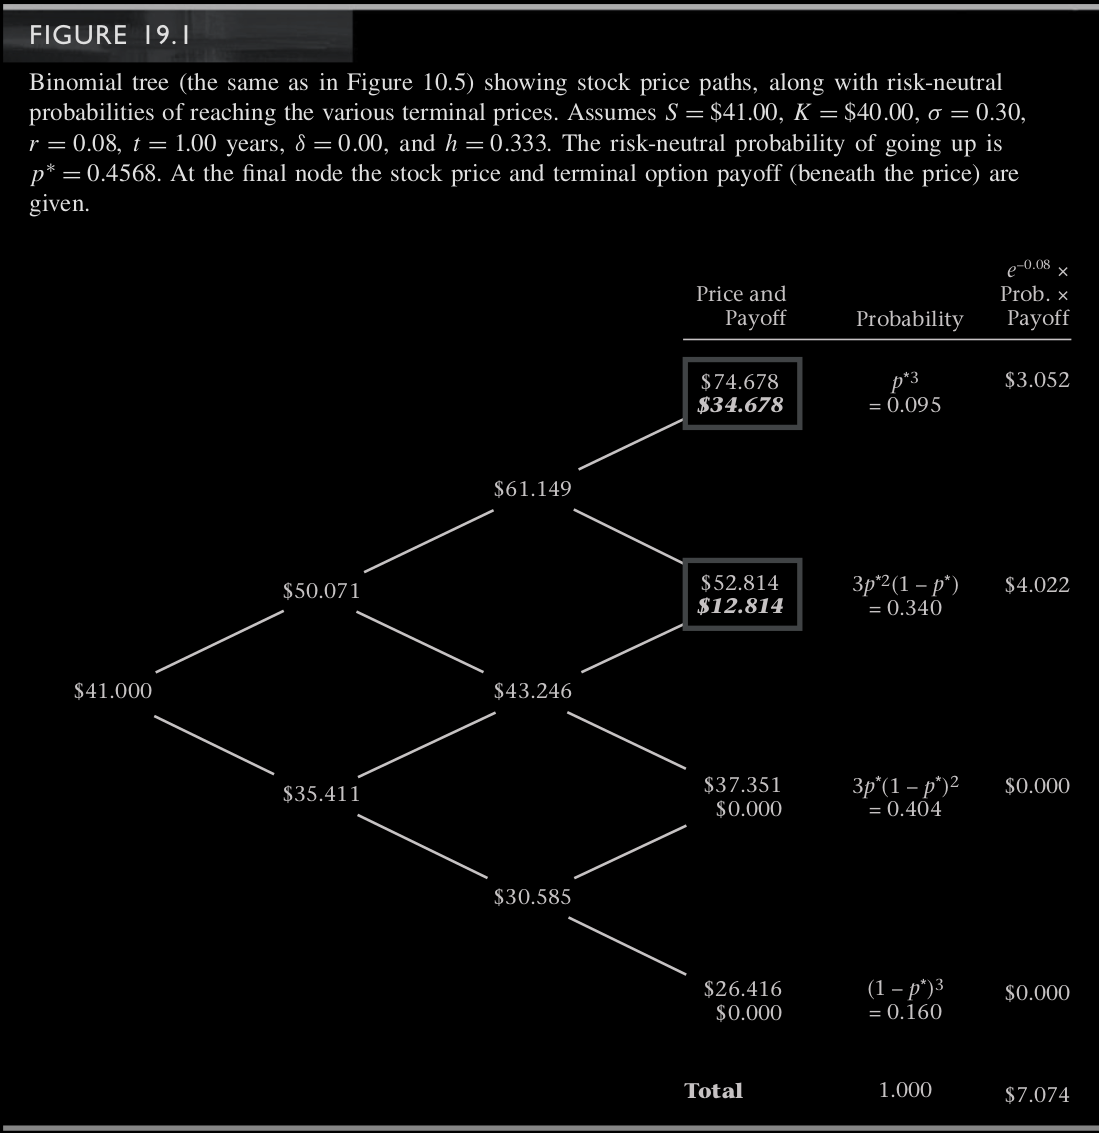
\includegraphics[scale=0.25]{figs/Figure_19-1.png}
\end{center}
\end{frame}
%-------------- end slide -------------------------------%}}}
%-------------- start slide -------------------------------%{{{ 1
\begin{frame}[fragile,t]
Instead of using the formula to compute the option price, one can simulate ...
\bigskip

\begin{myexample}
	Write a piece of code to simulate the binomial tree and compute the corresponding average payoff.
\end{myexample}
\bigskip
\begin{mysol}
	Check \\
	\begin{center}
		\textcolor{gray}{codes/Section\_19-1.py}
	\end{center}
	\myEnd
\end{mysol}
\end{frame}
%-------------- end slide -------------------------------%}}}

\def\mySecNum{19.2}
\mySection{\mySecNum~Computing random numbers}
%-------------- start slide -------------------------------%{{{ 1
\begin{frame}[fragile]
	\begin{center}
		Check out the \textcolor{magenta}{numpy.random} reference\footnote{There is no need to build
		the wheels by ourselves.} :
		\bigskip
		\bigskip

		\small
		\url{https://numpy.org/doc/1.16/reference/routines.random.html}
	\end{center}
\end{frame}
%-------------- end slide -------------------------------%}}}

\def\mySecNum{19.3}
\mySection{\mySecNum~Simulating lognormal stock prices}
%-------------- start slide -------------------------------%{{{ 1
\begin{frame}[fragile,t]
\begin{align*}
	S_T & = S_0 e^{\left(\alpha-\delta-\frac{1}{2}\sigma^2\right) T + \sigma \sqrt{T} Z}
\end{align*}
\mySeparateLine
\begin{align*}
	S_h    & = S_0 e^{\left(\alpha-\delta-\frac{1}{2}\sigma^2\right) h + \sigma \sqrt{h} Z_1}        \\
	S_{2h} & = S_h e^{\left(\alpha-\delta-\frac{1}{2}\sigma^2\right) h + \sigma \sqrt{h} Z_2}        \\
	\vdots & \qquad \qquad \vdots                                                                    \\
	S_{nh} & = S_{(n-1)h} e^{\left(\alpha-\delta-\frac{1}{2}\sigma^2\right) h + \sigma \sqrt{h} Z_n} \\
\end{align*}
\begin{align*}
	\Downarrow
\end{align*}
\begin{align*}
	S_{nh} & = S_0 e^{\left(\alpha-\delta-\frac{1}{2}\sigma^2\right) h + \sigma \sqrt{h} \sum_{i=1}^{n} Z_i}
	= S_0e^{\left(\alpha-\delta-\frac{1}{2}\sigma^2\right) h + \sigma \sqrt{T} \textcolor{magenta}{\left[\frac{1}{\sqrt{n}}\sum_{i=1}^{n} Z_i\right]}}
\end{align*}
\begin{center}
	where
\end{center}
\begin{align*}
	\textcolor{magenta}{\frac{1}{\sqrt{n}}\sum_{i=1}^{n} Z_i} \sim N\left(0,1\right)
\end{align*}
\end{frame}
%-------------- end slide -------------------------------%}}}

\def\mySecNum{19.4}
\mySection{\mySecNum~Monte Carlo valuation}
%-------------- start slide -------------------------------%{{{ 1 Expression in general
\begin{frame}[fragile,t]
	\begin{align*}
		V(S_0,0) = \frac{1}{n} e^{-rT}\sum_{n=1}^{n} V\left(S_T^i,T\right)
	\end{align*}
	where
	\begin{itemize}
		\item $S_T^1,\cdots, S_T^n$ are  $n$ randomly drawn time-$T$ stock prices.
		\item For European Call:
			\begin{align*}
				V(S_T^i,T) = \max\left(0,S_T^i-K\right)
			\end{align*}
		\item[] Similarly one finds the expression for European put.
	\end{itemize}
\end{frame}
%-------------- end slide -------------------------------%}}}
%-------------- start slide -------------------------------%{{{ 1 Table 19.2
\begin{frame}[fragile,t]
\begin{myexample}
	Carry out the Monte Carlo valuation of the European call under the setting of the following table:
	\begin{center}
		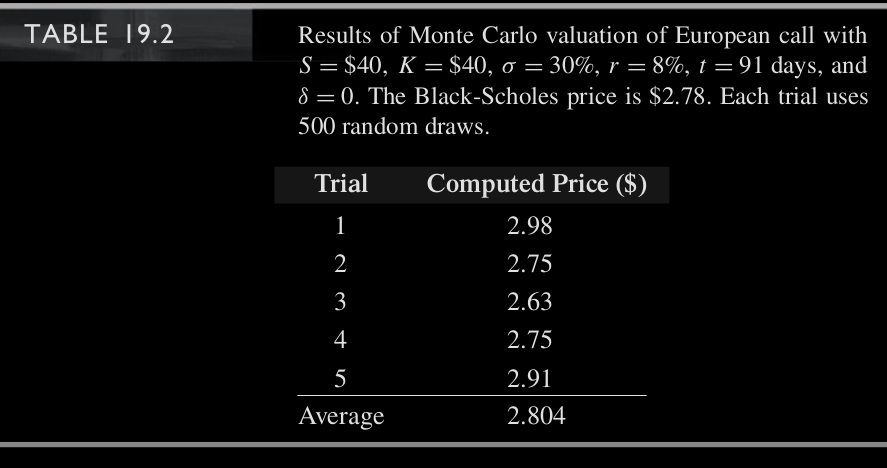
\includegraphics[scale=0.25]{figs/Table_19-2.png}
	\end{center}
\end{myexample}
\bigskip
\begin{mysol}
Check
\begin{center}
	\textcolor{gray}{codes/Table\_19-2.py}
\end{center}
\myEnd
\end{mysol}
\end{frame}
%-------------- end slide -------------------------------%}}}
%-------------- start slide -------------------------------%{{{ 1 Table 19.3
\begin{frame}[fragile,t]
\begin{myexample}
	Carry out the Monte Carlo valuation of the Asian call under the setting of the following table:
	\begin{center}
		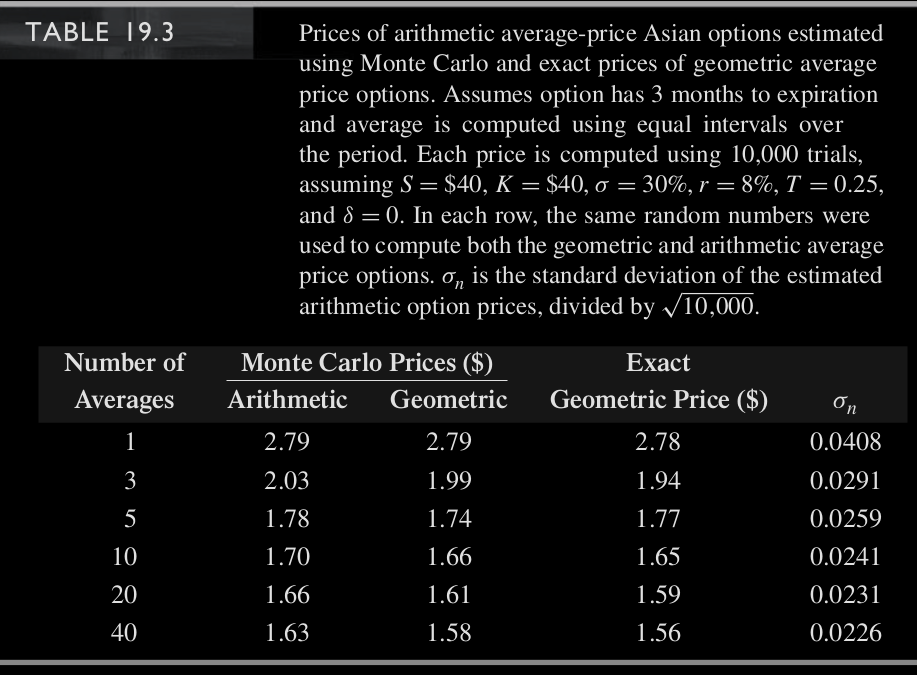
\includegraphics[scale=0.25]{figs/Table_19-3.png}
	\end{center}
\end{myexample}
\begin{mysol}
Check
\begin{center}
	\textcolor{gray}{codes/Table\_19-3.py}
\end{center}
\myEnd
\end{mysol}
\end{frame}
%-------------- end slide -------------------------------%}}}

\def\mySecNum{19.5}
\mySection{\mySecNum~Efficient Monte Carlo valuation}
%-------------- start slide -------------------------------%{{{ 1 Skip
\begin{frame}[fragile,t]
 \begin{center}
  This section will be skipped for the interested students.
\end{center}
\end{frame}
%-------------- end slide -------------------------------%}}}

\def\mySecNum{19.6}
\mySection{\mySecNum~Valuation of American options}
%-------------- start slide -------------------------------%{{{ 1 Skip
\begin{frame}[fragile,t]
 \begin{center}
  This section will be skipped for the interested students.
\end{center}
\end{frame}
%-------------- end slide -------------------------------%}}}

% \def\mySecNum{19.7}
\mySection{\mySecNum~The Poisson distribution}
%-------------- start slide -------------------------------%{{{ 1 Skip
\begin{frame}[fragile,t]
 \begin{center}
  This section will be skipped for the interested students.
\end{center}
\end{frame}
 %-------------- end slide -------------------------------%}}}

% \def\mySecNum{19.8}
\mySection{\mySecNum~Simulating jumps with the Poisson distribution}
%-------------- start slide -------------------------------%{{{ 1 Skip
\begin{frame}[fragile,t]
\begin{center}
This section will be skipped for the interested students.
\end{center}
\end{frame}
%-------------- end slide -------------------------------%}}}

% \def\mySecNum{19.9}
\mySection{\mySecNum~Simulating correlated stock prices}
%-------------- start slide -------------------------------%{{{ 1 Skip
\begin{frame}[fragile,t]
\begin{center}
	This section will be skipped for the interested students.
\end{center}	
\end{frame}
%-------------- end slide -------------------------------%}}}

% \def\mySecNum{19.10}
\mySection{\mySecNum~Problems}
%-------------- start slide -------------------------------%{{{ 1 Problems
\begin{frame}[fragile,t]
	Problems:
	19.5,
	19.6,
	19.7,
	19.8.
	% 10.15.
	% 5.11,
	% 5.12,
	% 5.16,
	% 5.20.
	\\
	\bigskip

	Due Date: TBA
\end{frame}
%-------------- end slide -------------------------------%}}}

\end{document}
